% !TEX root = ../masterthesis.tex
\chapter{Methods}

\todo{Einleitung}


\section{Optical setup}

The setup used for the measurements described in following chapters is sketched in figure~\ref{fig:setupflat}.

\begin{figure}[H]
	\centering
	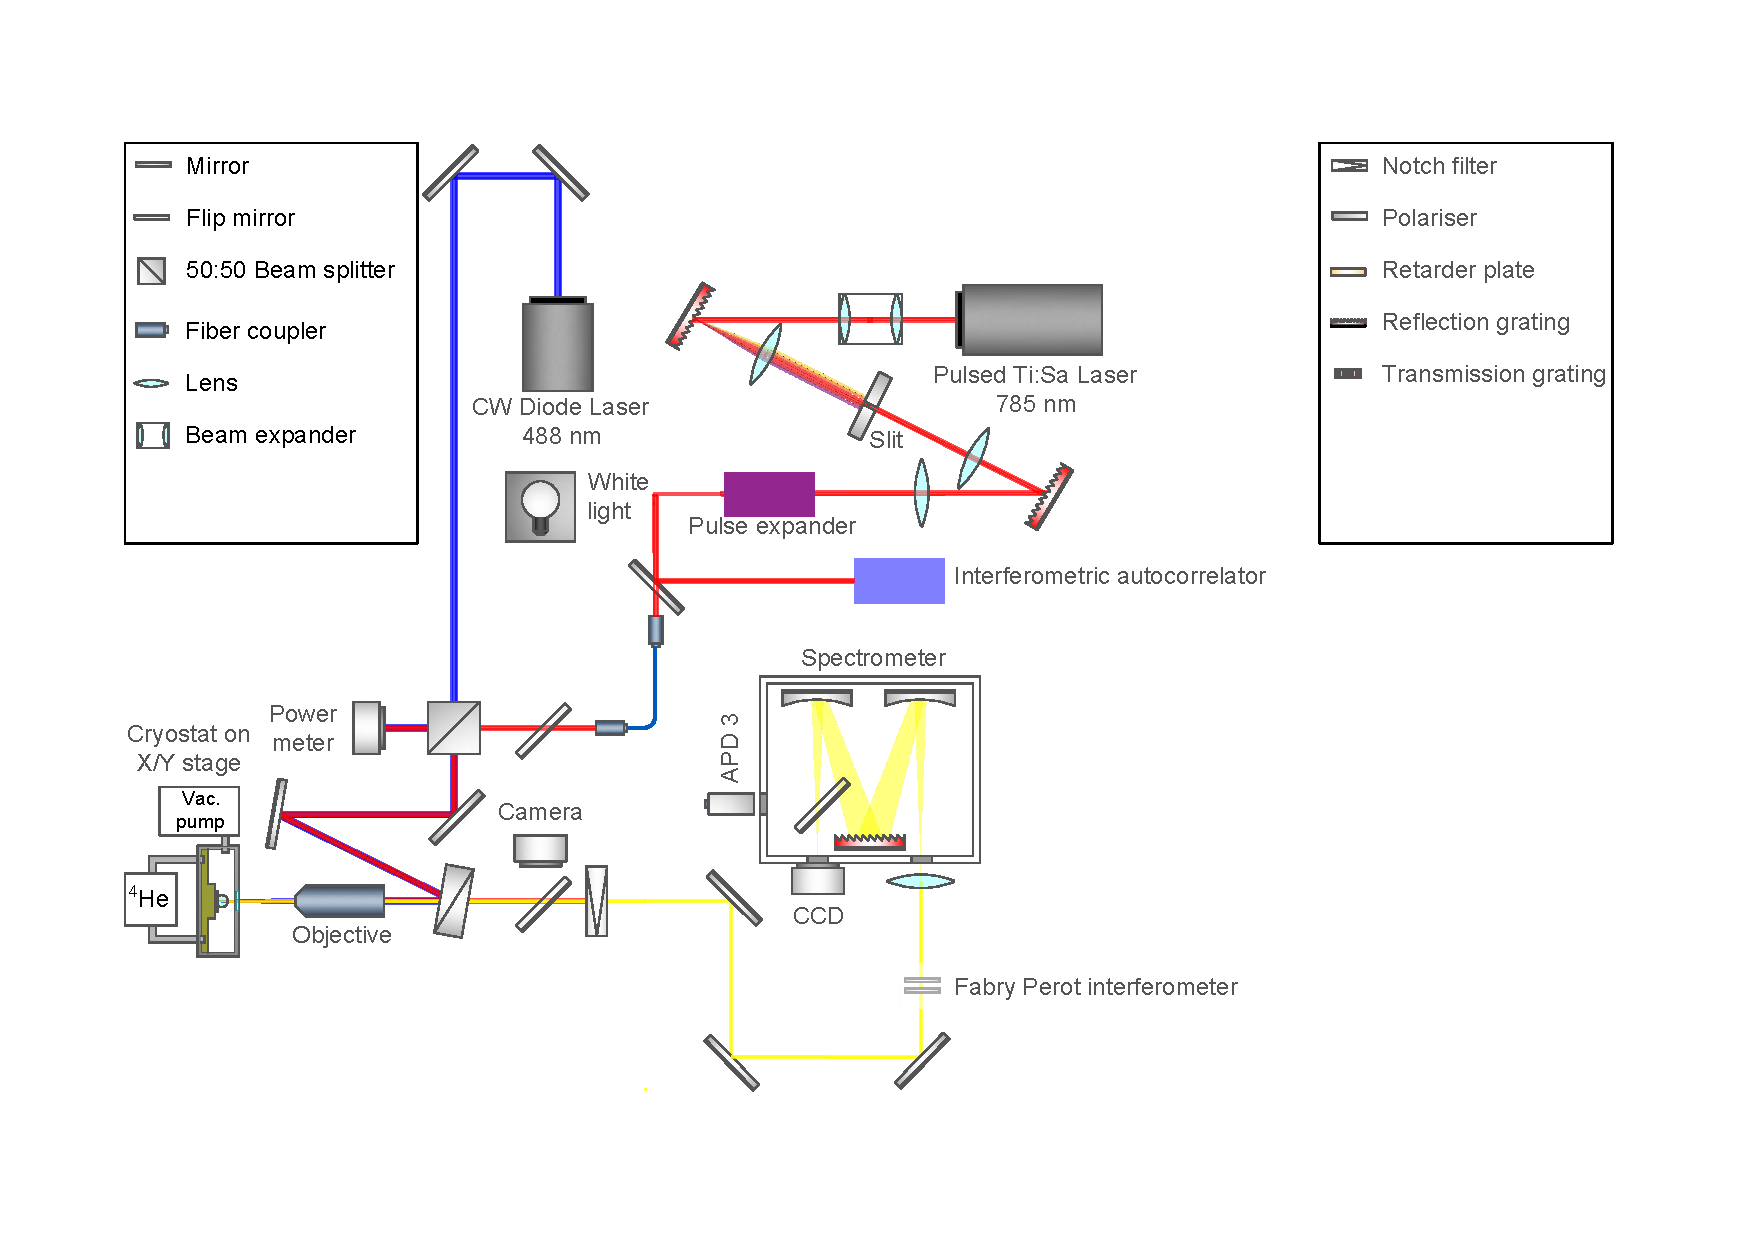
\includegraphics[width=\linewidth]{figures/setup/Setup_flat}
	\caption[Complete experimental setup]{Complete experimental setup, which was used in order to quantify the chirp of the Ti:Sa Laser and resolve spectral emission of a quantum dot~\cite{schimpf_towards_2017}.}
	\label{fig:setupflat}
\end{figure}

\todo{Pulse shaper 4F geometrie, florian sipek}
\todo{helium flow crystat 4K}

\section{Micro photo-luminescence}
\begin{figure}[H]
	\centering
	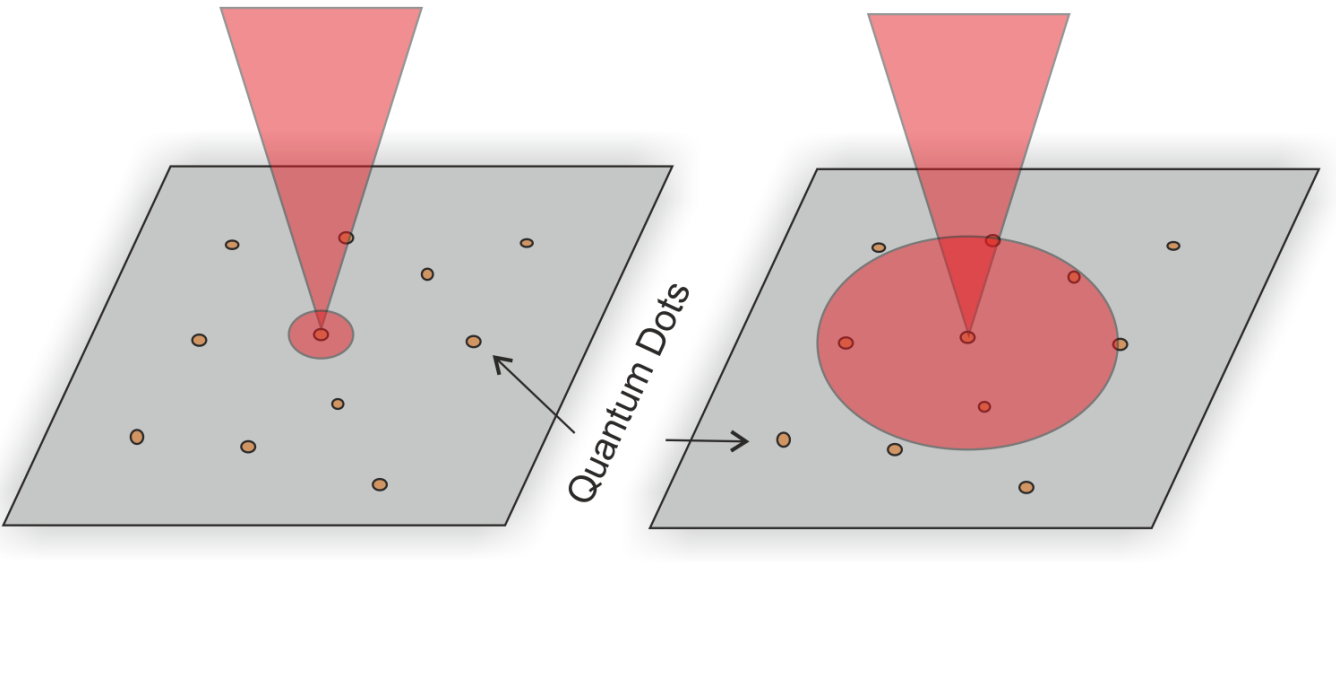
\includegraphics[width=0.7\linewidth]{figures/setup/micro-pl}
	\caption{Laser beam of different spot sizes illuminating quantum dots~\cite{reindl_characterisation_2014}.}
	\label{fig:micro-pl}
\end{figure}
The following chapters will investigate the optical properties of \ac{QD}.
In order to achieve that, it is necessary to excite and collect light of only a single one.
This is achieved by \ac{MPL}, which involves (i) reducing the diameter of the excitation laser beam and (ii) using samples with a low \ac{QD} density~\cite{reindl_characterisation_2014}.
(i) can be improved by using an objective, where its minimal achievable spot size $d$ is described by
\begin{equation}
d = \frac{\lambda}{2 \cdot NA}
\end{equation}
with $NA$ as the numerical aperture.
As the wavelength of the laser $\lambda$ is adjusted according parameter of the \ac{QD}, $NA$ is the adjustable factor.
In our laboratory, an objective of $NA=0.62$ is used, allowing laser spot sizes in the order of the excitation wavelength.
A \ac{QD} density of $\approx 1 / \lambda^2$ is therefore necessary in order to examine single \ac{QD} emission.

The sample containing the \acp{QD} is mounted inside the cryostat, which is cooled down to \SI{4}{\kelvin}.
This is necessary as the influence of dephasing processes increases with higher temperature due to carrier-phonon interaction.
The laser beam is then focused on the sample by the objective and the \ac{QD} emission is then collected by the very same objective and passed through a beam splitter.